\documentclass[12pt]{extarticle}
\usepackage[left = 2cm, right = 2cm, top = 2cm, bottom = 2cm]{geometry}
\usepackage{graphicx}
\usepackage{amsmath}
\usepackage{amssymb}
\usepackage{hyperref}
\usepackage{listings}
%\linespread{2}

\begin{document}

\begin{flushleft}
\begin{LARGE}
\textbf{2.4}
\end{LARGE}
\end{flushleft}

\vfill
\begin{center}
\begin{Huge}Simulation of Random Samples from Parametric Distributions\end{Huge}
\end{center}
\vfill

\pagebreak


\textbf{Question 1}

$$\int_{0}^{m}f(x|\theta)dx  = \int_{0}^{m}\theta e^{-\theta x} dx = \left[-e^{-\theta x} \right]_0^m  = 1-e^{-\theta m}$$

So $$1-e^{-\theta m} = \frac{1}{2} \Rightarrow \theta = \frac{\log2}{m}$$

$$g(x|m) = f(x|\theta(m)) = \frac{\log{2}}{m}\exp{\left(-\frac{x\log{2}}{m}\right)}$$

\textbf{Question 2}\\

We generate $\textbf{u}$ using the rand function on Matlab and calculate $\textbf{x}$ using $x_i = -\log(1-u_i)/\theta_0$.

$\textbf{u} = (0.1703, 0.5678, 0.8448, 0.3876, 0.6143, 0.5114)$

$\textbf{x} = (0.1555, 0.6991,1.5526, 0.4087 ,0.7940,0.5969)$

\begin{figure}[htp!]
\centering
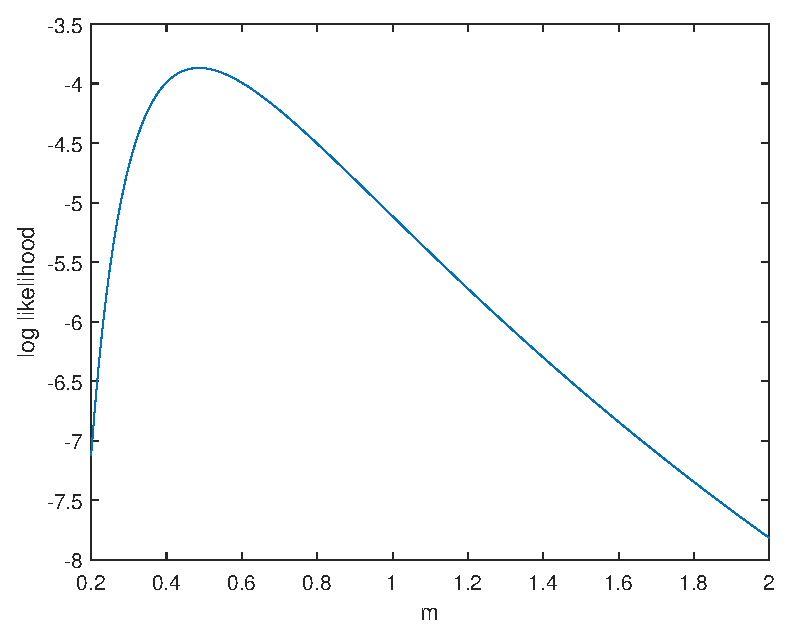
\includegraphics[scale=0.9]{loglike_Q2.eps}\\
\caption{log likelihood against m}
\label{figure:1}
\end{figure}

$$l_n(m) = \log{\prod_{i=1}^{n} g(x_i|m)} = \log{\left(\prod_{i=1}^{n} \frac{\log{2}}{m}\exp{\left(-\frac{x_i\log2}{m}\right)}\right)}$$ 

$$ = \log{\left(\left(\frac{\log2}{m}\right)^n \exp{\left(-\frac{\log2}{m}\sum_{i=1}^{n}x_i\right)}\right)} =n\log{\left(\log{2}\right)} -n\log{m} -\frac{\log{2}}{m}\sum_{i=1}^{n}x_i$$

Differentiating w.r.t $m$ and setting equal to zero

$$-\frac{n}{m} + \frac{\log{2}}{m^2}\sum_{i=1}^{n}x_i = 0 \Rightarrow \widehat{m}_n = \bar{x}\log{2}$$

From the plot the function takes its maximum value at $m = 0.48$. Using the above derivation, $\widehat{m}_6 = \bar{x}\log{2} = 0.4860$ so the two results agree. The true value of the median is $m_0 = \log{2}/\theta_0 = \log{2}/1.2 = 0.578$.

$$\mathbb{E}(\widehat{m}_n) = \mathbb{E}(\bar{X}\log2) = \frac{\log2}{n}\sum_{i=1}^{n}\mathbb{E}(X_i) = \frac{\log{2}}{\theta_0} = m_0$$

So $\widehat{m}_n$ is an unbiased estimator of $m_0$.\\

\textbf{Question 3}\\

$\underline{n = 25}$

$\textbf{u} = (0.1071,0.5032,0.3048 ,\ldots ,0.1207,0.7771, 0.9623
)$

$\textbf{x} = (0.0944,0.5829,0.3030 ,\ldots, 0.1072,1.2510,2.7307)$

$\widehat{m}_{25} = 0.6585$\\


$\underline{n = 50}$

$\textbf{u} = (0.3924,0.6756, 0.2969, \ldots, 0.4408,0.7000,0.6092)$

$\textbf{x} = (0.4152,0.9382,0.2935, \ldots, 0.4843,  1.0034, 0.7829)$

$\widehat{m}_{50} = 0.6559$\\


$\underline{n = 100}$

$\textbf{u} = (0.3932,0.1330, 0.6493, \ldots, 0.6227, 0.2867, 0.9085)$

$\textbf{x} = (0.4163,0.1189,0.8731, \ldots, 0.8122,0.2816, 1.9933)$

$\widehat{m}_{100} = 0.5857$

\begin{figure}[htp!]
\centering
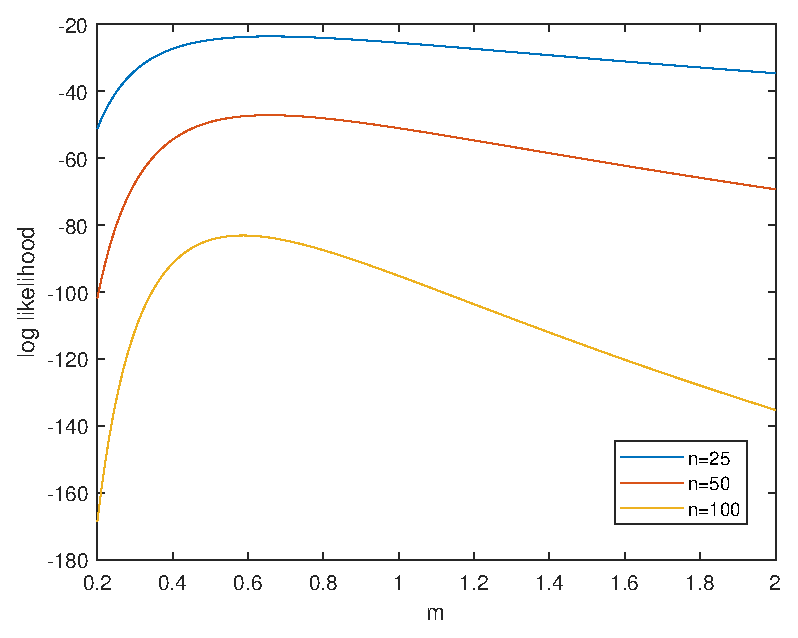
\includegraphics[scale=0.9]{loglike_Q3.eps}
\caption{\textit{log likelihood} against $m$}
\label{figure:2}
\end{figure}

\pagebreak 

$$\mathrm{var}(\widehat{m}_n) = \mathrm{var}(\bar{X}\log2) = \frac{(\log2)^2}{n^2}\sum_{i=1}^{n}\mathrm{var}(X_i) = \frac{1}{n}\left(\frac{\log2}{\theta_0}\right)^2 = \frac{m_0^2}{n}$$

$$l_n(\widehat{m}_n) = n\log{\left(\log{2}\right)} -n\log{\widehat{m}_n} -\frac{\log{2}}{\widehat{m}_n}\sum_{i=1}^{n}x_i = -n\log\bar{x}-\frac{1}{\bar{x}}\sum_{i=1}^{n}x_i = -n(\log\bar{x}+1)$$

The peaks of the plots occur at values of $m$ close to $m_0$  $(0.578)$, agreeing with the expected value. The maximum of the \textit{log likelihood} plots decreases in accordance with the calculation above.  The range of the \textit{log likelihood} also increases with $n$ and the peaks become steeper. This demonstrates that the variance of $\widehat{m}_n$ decreases as $n$ increases - it becomes more probable to obtain a value of $m$ close to $\widehat{m}_n$ as $n$ increases.\\

\textbf{Question 4}\\

The moment generating function of $X$ is 
$$M_X(\lambda) = \mathbb{E}(e^{\lambda X}) = \int_{0}^{\infty} \theta e^{-\theta x}e^{\lambda x}dx = \int_{0}^{\infty} \theta e^{(\lambda-\theta) x}dx =\left[ \frac{\theta}{\lambda-\theta}e^{(\lambda-\theta) x} \right]_0^\infty = \frac{\theta}{\theta - \lambda} = (1-\lambda/\theta)^{-1}, \lambda < \theta$$

The moment generating function of $X+Y$ is 
$$M_{X+Y}(\lambda) = \mathbb{E}(e^{\lambda (X+Y)}) = \mathbb{E}(e^{\lambda X})\mathbb{E}(e^{\lambda Y}) = M_X(\lambda)M_Y(\lambda) = (1-\lambda/\theta)^{-1}(1-\lambda/\theta)^{-1} =  (1-\lambda/\theta)^{-2}$$

Therefore $X+Y \sim \Gamma(2,\theta)$, by the uniqueness of moment generating functions. \\

\textbf{Question 5}
$$F(x) = \int_{0}^{x}\theta^2te^{-\theta t}dt = \left[-\theta t e^{-\theta t} \right]_0^x + \int_{0}^{x}\theta e^{-\theta t} dt = -\theta x e^{-\theta x} + \left[-e^{-\theta t} \right]_0^x = 1 - e^{-\theta x} - \theta x e^{-\theta x}$$

The Lambert $W$ function, defined as the inverse to the function $f(x) = xe^x$, will be used to compute $F^{-1}$. Let $u = F(x)$

$$u = 1-e^{-\theta x} - \theta x e^{-\theta x}$$
$$1-u = (1+\theta x)e^{-\theta x}$$

Now let $z = -1- \theta x$

$$1-u = -ze^{1+z}$$
$$\frac{u-1}{e} = ze^z$$
$$z = W\left(\frac{u-1}{e}\right)$$
$$x = -\frac{1}{\theta}\left(W\left(\frac{u-1}{e}\right)+1\right) = F^{-1}(u)$$\\

\textbf{Question 6}
$$l_n(\theta) = \log{\prod_{i=1}^{n} f(x_i|\theta)} = \log{\prod_{i=1}^{n}\theta^2x_ie^{-\theta x_i}} = \log{\theta^{2n}}+\log{\prod_{i=1}^{n}x_i}+\log{\left(\exp{\left(-\theta\sum_{i=1}^{n}x_i\right)}\right)}$$
$$ = 2n\log{\theta} +\log{\prod_{i=1}^{n}x_i}-\theta\sum_{i=1}^{n}x_i$$

Differentiating w.r.t $\theta$ and setting equal to zero

$$\frac{2n}{\theta}- \sum_{i=1}^{n}x_i = 0 \Rightarrow \widehat{\theta} = \frac{2}{\bar{x}}$$

\textbf{Question 7}

\underline{n=10}

$\textbf{u} = (0.7849,0.9365,0.8917,0.3359,0.6191, 0.4655, 0.1213,0.9362,0.5287,0.9121)$

$\textbf{x} = (1.3168,2.0241,1.7226,0.5436,0.9523, 0.7139,0.2720 ,2.0212 ,0.8053 ,1.8416)$

$\hat{\theta}_{10} = 1.6375$\\

\underline{n=30}

$\textbf{u} = (0.2384,
    0.3230,
    0.6421,
    \ldots,
    0.4885,
    0.7936,
    0.5752)$

$\textbf{x} = (0.4226,
   0.5275,
   0.9938,
   \ldots,
   0.7463,
   1.3420,
   0.8780)$

$\hat{\theta}_{30} = 2.3143$\\

\underline{n=50}

$\textbf{u} = (0.4757,
    0.5381,
    0.0402
    \ldots
    0.9554,
    0.6950,
    0.1514)$

$\textbf{x} = (0.7282,
    0.8196,
    0.1429
    \ldots
    2.2188,
    1.0982,
    0.3124)$

$\hat{\theta}_{50} =2.2027$

\begin{figure}[htp!]
\centering
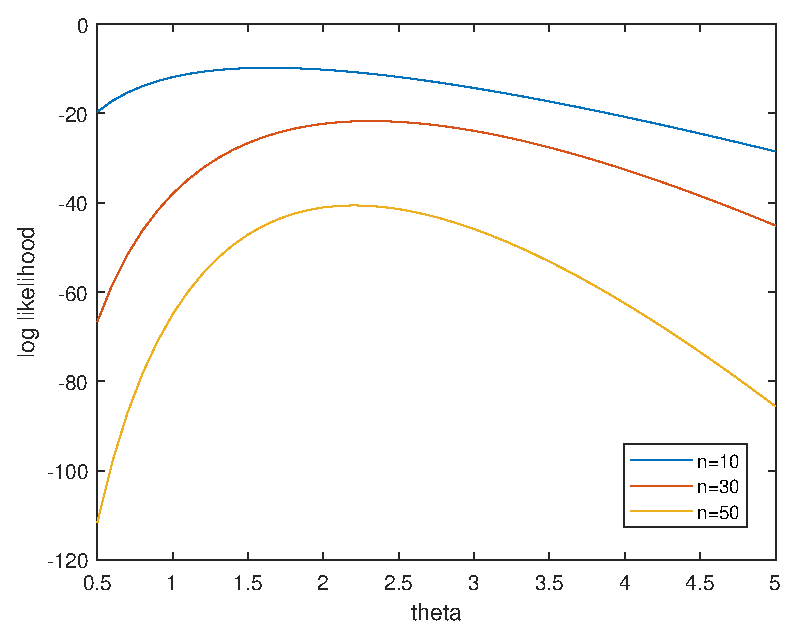
\includegraphics[scale=0.83]{loglike_Q7.eps}\\
\caption{\textit{log likelihood} against $\theta$}
\label{figure:3}
\end{figure}

As $n$ increases $\widehat{\theta}_n$ gets closer to $\theta_0$, presumably since its expected value is $\theta_0$ (2.2). Also $\widehat{\theta}_n$ is closer to $\theta_0$ than $\widehat{m}_n$ is to $m_0$ in Q3, possibly since $\widehat{\theta}_n$ has variance which decreases more quickly with $n$. The peaks again become steeper as $n$ increases since the variance decreases. \\

\textbf{Question 8}

\begin{figure}[htp!]
\centering
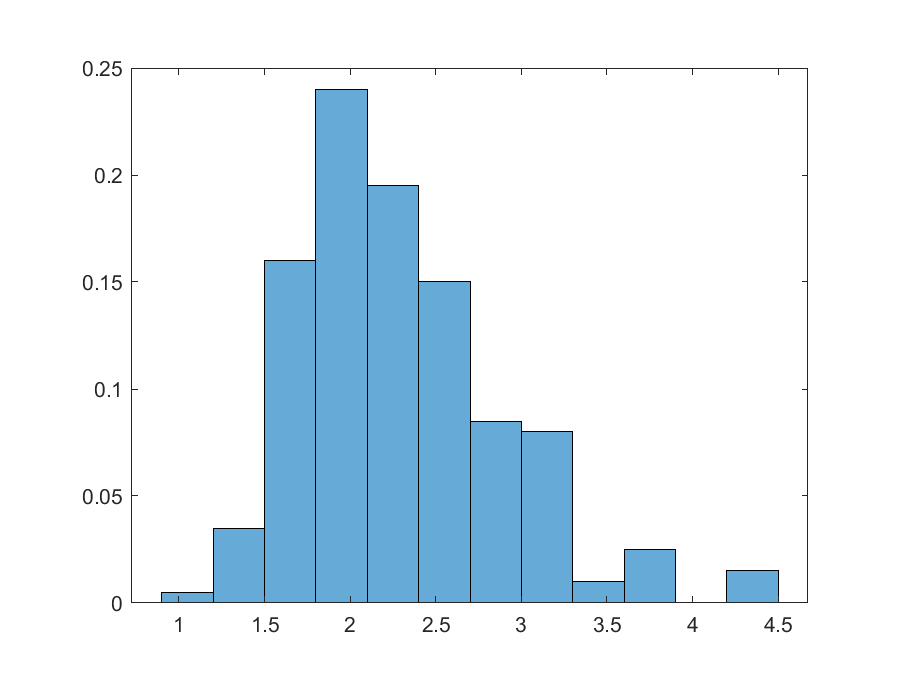
\includegraphics[scale=0.8]{histogram_Q8_10.eps}\\
\caption{Histogram of $\widehat{\theta}_n$ for $n=10$}
\label{figure:4}
\end{figure}

\begin{figure}[htp!]
\centering
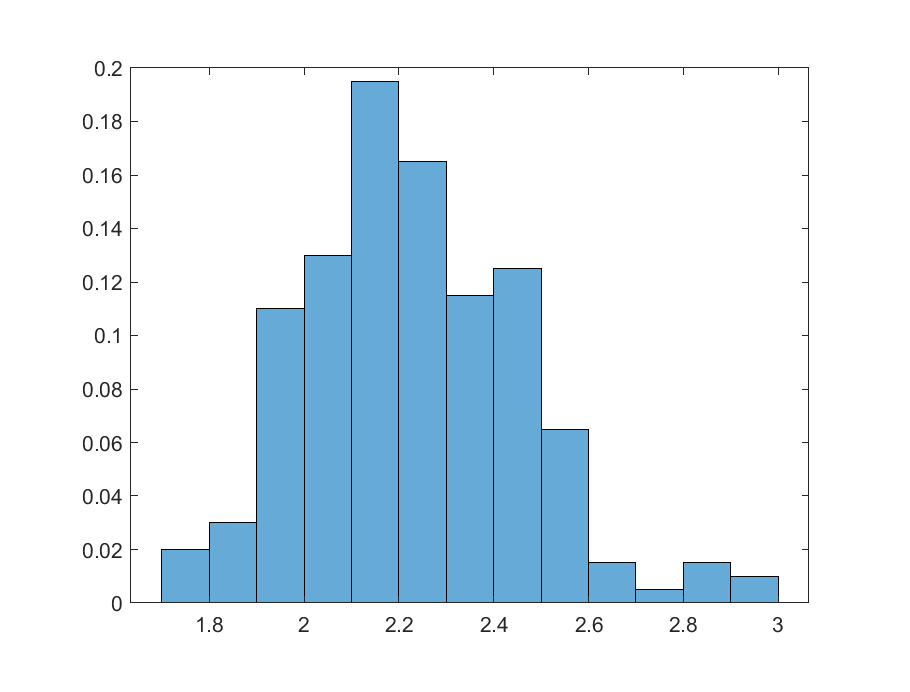
\includegraphics[scale=0.8]{histogram_Q8_50.eps}\\
\caption{Histogram of $\widehat{\theta}_n$ for $n=50$}
\label{figure:5}
\end{figure}

The histograms have been normalised to display the p.d.f of $\widehat{\theta}_n$. The range of values that $\widehat{\theta}_n$ takes decreases as we increase $n$ to 50, since its variance decreases. There is a greater probability density close to $\theta_0$, which suggests that it is indeed the expected value. Both histograms have a slight positive skew.\\

\textbf{Question 9}\\

Need to show the map is a bijection $(\Phi, V) \leftrightarrow (X,Y)$.

$$X = \mu_1 + \sigma \sqrt{V}\cos{\Phi},\;Y = \mu_2 + \sigma \sqrt{V}\sin{\Phi}$$

$$V = \left(\frac{X-\mu_1}{\sigma}\right)^2+\left(\frac{Y-\mu_2}{\sigma}\right)^2,\;\tan{\Phi} = \frac{Y-\mu_2}{X-\mu_1}$$

Where $\Phi$ is defined as the angle from the positive $X$ axis to the position vector $(X-\mu_1,Y-\mu_2)$. 

There is a bijection so the theorem can be used.

$$\frac{\partial{x}}{\partial{v}} = \frac{1}{2}\sigma v^{-1/2}\cos{\phi} ,\; \frac{\partial{y}}{\partial{v}} = \frac{1}{2}\sigma v^{-1/2}\sin{\phi}$$ 

$$\frac{\partial{x}}{\partial{\phi}} = -\sigma v^{1/2}\sin{\phi},\;\frac{\partial{y}}{\partial{\phi}} =\sigma v^{1/2}\cos{\phi}$$

$$\left|\frac{\partial(x,y)}{\partial(v,\phi)}\right| =
\left|\frac{\partial{x}}{\partial{v}}\frac{\partial{y}}{\partial{\phi}}-\frac{\partial{y}}{\partial{v}}\frac{\partial{x}}{\partial{\phi}}\right| = 
\frac{1}{2}\sigma^2\cos^2{\phi} + \frac{1}{2}\sigma^2\sin^2{\phi} = \frac{1}{2}\sigma^2
$$

The theorem will be used in reverse
$$f(\phi,v) = g(x,y)\left|\frac{\partial(x,y)}{\partial(\phi,v)}\right|$$
$$g(x,y) = \frac{2}{\sigma^2}f(\phi(x,y), v(x,y)) = \frac{2}{\sigma^2}\frac{1}{4\pi}e^{-v(x,y)/2} = \frac{1}{2\pi\sigma^2}e^{-((x-\mu_1)^2+(y-\mu_2)^2)/2\sigma^2}$$

with $-\infty < x,y < \infty$, since $v \geq 0$ and $-1\leq \cos{\phi}, \sin{\phi} \leq 1$.\\

\textbf{Question 10}\\

The histogram below looks like a normal distribution so the program works.\\

The 80\% confidence interval will be constructed using $\bar{X}$. $X_1, \ldots, X_n \sim N(\mu, 1)$ independently so $\bar{X} \sim N(\mu, 1/n)$. If $a$ and $b$ are such that $\mathbb{P}(a \leq N(0,1) \leq b) = 0.8$,

$$\mathbb{P}(a \leq \sqrt{n}(\bar{X}-\mu) \leq b) = 0.8$$
$$\mathbb{P}(\bar{X}-\frac{b}{\sqrt{n}} \leq \mu \leq \bar{X}-\frac{a}{\sqrt{n}}) = 0.8$$

The symmetry of the normal distribution implies that $a$ and $b$ should be symmetric about 0.

$$\mathbb{P}(-b \leq N(0,1) \leq b) = 0.8$$ 
$$\mathbb{P}(N(0,1) \leq b) = 0.9$$
$$b = \Phi^{-1}(0.9) = 1.28$$  

So an 80\% confidence interval for $\mu$ is $\left[\bar{X}-1.28/\sqrt{n},\bar{X}+1.28/\sqrt{n}\right]$.\\

\begin{figure}[htp!]
\centering
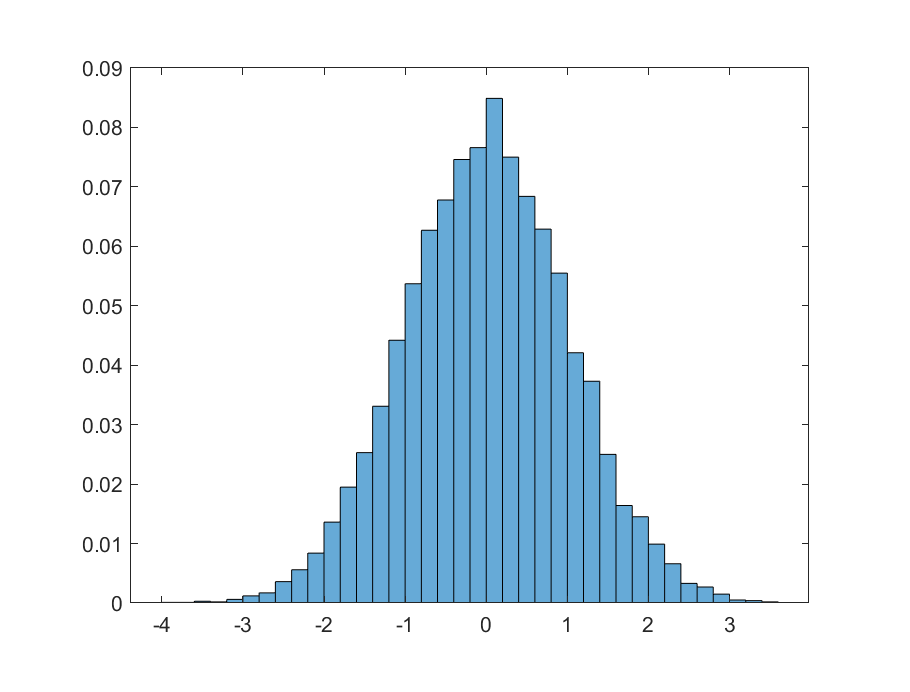
\includegraphics[scale=0.9]{histogram_Q10.eps}\\
\caption{Normalised histogram of $(x_1, \ldots, x_n)$ for $n = 10000$ }
\label{figure:6}
\end{figure} 

\textbf{Question 11}\\

$\textbf{x} = (1.5264,
   -0.5797,
    1.2837,
    \ldots,
    0.1128,
   -1.6924,
    1.0625)$

$\bar{x} = 0.1785 $

C.I. $= \left[\bar{x}-1.28/\sqrt{100},\bar{x}+1.28/\sqrt{100}\right] = [0.0505,0.3065]$

So $\mu = 0$ is not in the confidence interval. \\

The results are displayed in Table 1. The interval did not contain $\mu$ three times. Since it is an 80\% confidence interval, it is expected \textit{not} to contain $\mu$ 5 out of 25 times (20\%).\\
 
\textbf{Question 12}\\

It is still an 80\% confidence interval so is expected to contain the mean 80\% of the time and hence not to contain it 20\% of the time. If 25 trials are conducted then we expect 5 of them not to contain it. Indeed repeating the procedure with $n =50$ and $\mu = 4$ (Table 2) gives 4 intervals that did not contain the mean. Changing $\mu$ does not make a difference. Decreasing $n$ from 100 to 50 means $\bar{X}$ has a greater variance and so it is expected that there will be more deviation from 5 in the number of intervals not containing $\mu$.\\

\textbf{Question 13}\\

Let $k$ denote the number of degrees of freedom. $\chi^2_k = \Gamma(k/2, 1/2)$\footnote{$N(0,1)^2$ has m.g.f $(1-2t)^{-1/2}$ so $\chi^2_k$ has m.g.f $(1-2t)^{-k/2}$} so its expectation and variance can be found.
\begin{itemize}
\item $\mathbb{E}(\chi^2_k) = k/2(1/2)^{-1} = k$. The histograms move to the left as $k$ increases since the mean of the distribution increases. 
\item $\mathrm{var}(\chi^2_k) = k/2(1/2)^{-2} = 2k$. The histograms become broader and shorter. The variance increases which causes them to spread out. 
\item The skewness\footnote{\url{https://en.wikipedia.org/wiki/Chi-squared_distribution}} of $\chi^2_k$ is $\sqrt{8/k}$. The distributions $k = 1$ and $k=5$ have a positive skew. However the histograms become less skewed as $k$ increases (more symmetric). 
\item As $k \rightarrow \infty$, $\chi^2_k$ tends to a normal distribution, by the central limit theorem. This is evident in the case $k=40$, where the distributions (especially $n=500$) resemble a normal distribution. 
\end{itemize}

The histograms have been normalised to show the probability distributions. Increasing $n$ increases the number of variables in the sample, meaning the histograms can be plotted using smaller bin widths, as more values are taken by the variables. This makes them smoother and more like continuous probability density functions. 

\begin{figure}[htp!]
\centering
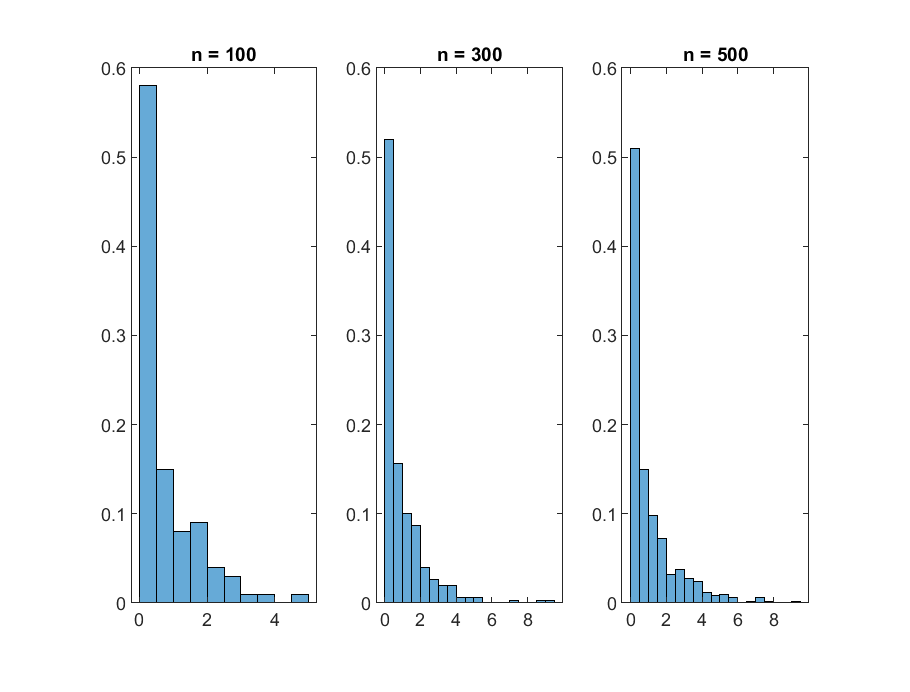
\includegraphics[scale=0.9]{histogram_Q13_1.eps}\\
\caption{Chi-square with 1 degree of freedom }
\label{figure:7}
\end{figure} 

\begin{figure}[htp!]
\centering
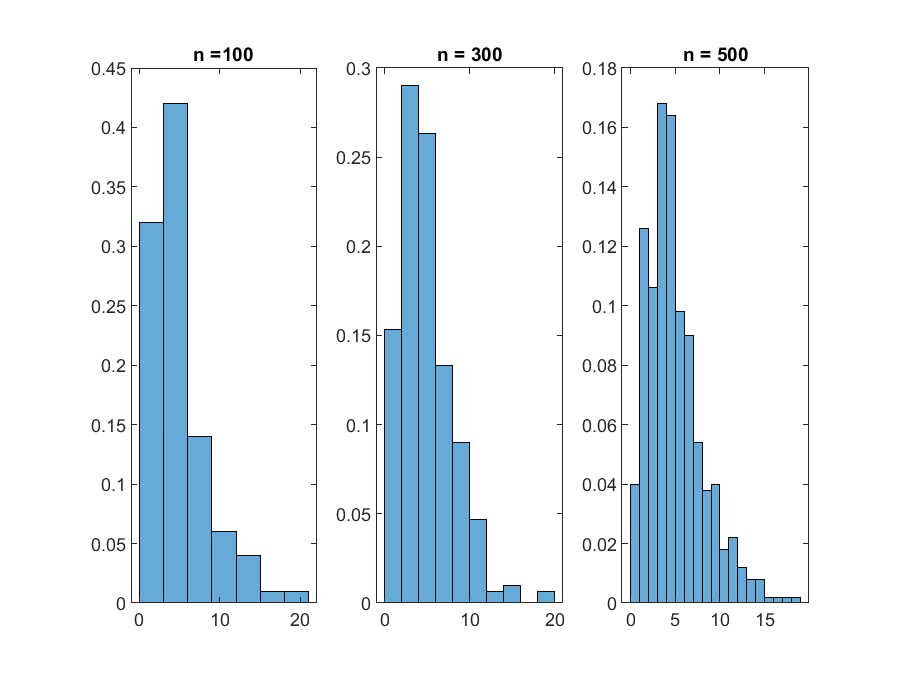
\includegraphics[scale=0.9]{histogram_Q13_5.eps}\\
\caption{Chi-square with 5 degrees of freedom }
\label{figure:8}
\end{figure} 

\begin{figure}[htp!]
\centering
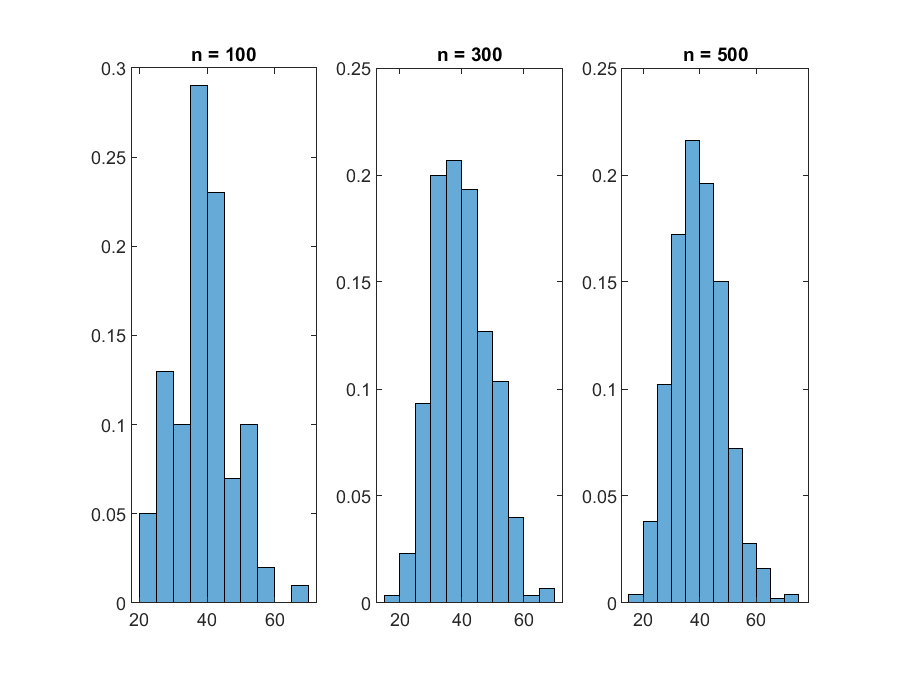
\includegraphics[scale=0.9]{histogram_Q13_40.eps}\\
\caption{Chi-square with 40 degrees of freedom }
\label{figure:9}
\end{figure} 

\begin{table}[h!]
\caption{Mean and Confidence Interval for samples from $\mu = 0$ and $n=100$}
\centering
\begin{tabular}{cccc}
\\
$\bar{x}$ & Lower Bound & Upper Bound & 0 or 1 \\ [0.5ex]
0.1151 & -0.0129 & 0.2431 & 1 \\ 
0.0462 & -0.0818 & 0.1742 & 1 \\ 
-0.1104 & -0.2384 & 0.0176 & 1 \\ 
0.0375 & -0.0905 & 0.1655 & 1 \\ 
-0.0258 & -0.1538 & 0.1022 & 1 \\ 
0.0601 & -0.0679 & 0.1881 & 1 \\ 
0.0214 & -0.1066 & 0.1494 & 1 \\ 
-0.0683 & -0.1963 & 0.0597 & 1 \\ 
-0.0583 & -0.1863 & 0.0697 & 1 \\ 
-0.0367 & -0.1647 & 0.0913 & 1 \\ 
0.0307 & -0.0973 & 0.1587 & 1 \\ 
0.0148 & -0.1132 & 0.1428 & 1 \\ 
-0.0245 & -0.1525 & 0.1035 & 1 \\ 
-0.0193 & -0.1473 & 0.1087 & 1 \\ 
0.0494 & -0.0786 & 0.1774 & 1 \\ 
-0.1781 & -0.3061 & -0.0501 & 0 \\ 
-0.1246 & -0.2526 & 0.0034 & 1 \\ 
-0.0522 & -0.1802 & 0.0758 & 1 \\ 
-0.1252 & -0.2532 & 0.0028 & 1 \\ 
-0.0242 & -0.1522 & 0.1038 & 1 \\ 
0.0506 & -0.0774 & 0.1786 & 1 \\ 
-0.1674 & -0.2954 & -0.0394 & 0 \\ 
0.0111 & -0.1169 & 0.1391 & 1 \\ 
-0.2272 & -0.3552 & -0.0992 & 0 \\ 
0.1206 & -0.0074 & 0.2486 & 1 \\
\end{tabular}
\label{table:1}
\end{table}

\begin{table}[h!]

\caption{Mean and Confidence Interval for samples from $\mu = 4$ and $n=50$}
\centering
\begin{tabular}{cccc}
\\
$\bar{x}$ & Lower Bound & Upper Bound & 0 or 1 \\ [0.5ex]
4.1665 & 3.9855 & 4.3476 & 1 \\ 
3.9940 & 3.8129 & 4.1750 & 1 \\ 
4.1669 & 3.9858 & 4.3479 & 1 \\ 
4.2088 & 4.0278 & 4.3899 & 0 \\ 
3.9264 & 3.7454 & 4.1074 & 1 \\ 
\vdots & \vdots & \vdots & \vdots \\
4.3042 & 4.1232 & 4.4853 & 0 \\ 
3.9389 & 3.7578 & 4.1199 & 1 \\ 
3.8307 & 3.6497 & 4.0117 & 1 \\ 
4.0235 & 3.8425 & 4.2046 & 1 \\ 
4.0672 & 3.8861 & 4.2482 & 1 \\ 
\end{tabular}
\label{table:2}
\end{table}
\pagebreak

\begin{center}
\textbf{Code for Q2,3}
\end{center}
\lstinputlisting[language=Matlab]{Q2_3.m}

\begin{center}
\textbf{Log likelihood function 1}
\end{center}
\lstinputlisting[language=Matlab]{loglike1.m}

\begin{center}
\textbf{Code for Q7}
\end{center}
\lstinputlisting[language=Matlab]{Q7.m}

\begin{center}
\textbf{Log likelihood function 2}
\end{center}
\lstinputlisting[language=Matlab]{loglike2.m}
\pagebreak

\begin{center}
\textbf{Code for Q8}
\end{center}
\lstinputlisting[language=Matlab]{Q8.m}

\begin{center}
\textbf{Code for Q10}
\end{center}
\lstinputlisting[language=Matlab]{Q10.m}

\begin{center}
\textbf{Code for Q11}
\end{center}
\lstinputlisting[language=Matlab]{Q11.m}

\begin{center}
\textbf{Code for Q13}
\end{center}
\lstinputlisting[language=Matlab]{Q13.m}

\end{document}
